\section{The leading family and an eta quotient}\label{sec:model}

Fix $m\ge1$ and a charge $(m,n,\ell)$ with $0\le\ell\le m$ and $D>0$; write $x=\sqrt D/m$, $\theta=\pi\ell/m$ and $t_0=m^2+4m$. The \emph{extreme term} is
\begin{equation}\label{eq:ext}
\mathcal E(D,m)=\frac{\pi}{\sqrt{2m}}\cdot\frac{m+2}{16}\Big(\frac{t_0}D\Big)^{\frac{15}4}I_{\frac{15}2}\big(\pi x\sqrt{t_0}\big)>0 .
\end{equation}
It is the contribution to $\frac12(-1)^\ell\sqrt i\,\mathcal M$ of the frame $S$, $\gamma=1$, and the most polar term $\tilde\nu=-1$, $\tilde\ell=m$, whose only wall is $G_0=\begin{psmallmatrix}1&0\\1&1\end{psmallmatrix}$ with $m_{G_0}=n_{G_0}=-1$ and $\ell_{G_0}=m+2$.

\subsection{The terms with \texorpdfstring{$\gamma=1$}{gamma=1}}
For $\gamma=1$ the set $\mathcal C_1$ consists of $\delta=0$ and $\delta=-1$, both with $\alpha=0$ and $\beta=-1$. The matrix $\begin{psmallmatrix}0&1\\-1&0\end{psmallmatrix}$ has frame $S$, and $\begin{psmallmatrix}-1&1\\-1&0\end{psmallmatrix}$ has frame $T$. So the terms with $\gamma=1$ are one term in frame $S$ and one in frame $T$.

In frame $S$, $W_{1,0}(\tilde\ell,\ell)=(2mi)^{-1/2}\e(-\ell\tilde\ell/2m)$ and the phase in \eqref{eq:radmain} is $1$. Since $\sqrt i/\sqrt{2mi}=1/\sqrt{2m}$,
\begin{equation}\label{eq:gamma1S}
\tfrac12(-1)^\ell\sqrt i\,\mathcal M_{\gamma=1,S}=\frac{\pi}{\sqrt{2m}}\sum_{(\tilde\nu,\tilde\ell)}a_S(\tilde\nu,\tilde\ell)\,(-1)^\ell\e\Big(-\frac{\ell\tilde\ell}{2m}\Big)\Big(\frac tD\Big)^{\frac{15}4}I_{\frac{15}2}(\pi x\sqrt t),\qquad t=-\tilde D .
\end{equation}
Split $a_S=a_S^{\rm lead}+a_S^{\rm rest}$, where $a_S^{\rm lead}$ is the term of $G_0$ in \eqref{eq:P0} and $a_S^{\rm rest}$ the sum over the walls with $rs\ge2$. Lemma~\ref{lem:walls}(vii) identifies the polar terms carrying $G_0$ with the set
\[
\mathcal L_m=\big\{(a,b)\in\ZZ^2:\ a,b\ge-1,\ k=m-a-b\ge1,\ t_{a,b}=k^2-4ab>0,\ -m\le b-a<m\big\},
\]
by $\tilde\nu=b$, $\tilde\ell=m+b-a$, with $a_S^{\rm lead}=\frac1{16}k\,d_1(a)d_1(b)$ and $t=t_{a,b}$. For $(a,b)\in\mathcal L_m$ put $S=a+b+2$ and
\begin{equation}\label{eq:rho}
\rho_{a,b}(x)=\frac{k}{m+2}\Big(\frac{t_{a,b}}{t_0}\Big)^{\frac{15}4}\frac{I_{15/2}(\pi x\sqrt{t_{a,b}})}{I_{15/2}(\pi x\sqrt{t_0})}.
\end{equation}

\begin{theorem}\label{thm:model}
The leading part of \eqref{eq:gamma1S} is
\begin{equation}\label{eq:leadsum}
\begin{split}
&\frac{\pi}{\sqrt{2m}}\sum_{(\tilde\nu,\tilde\ell)}a^{\rm lead}_S(\tilde\nu,\tilde\ell)\,(-1)^\ell\e\Big(-\frac{\ell\tilde\ell}{2m}\Big)\Big(\frac tD\Big)^{\frac{15}4}I_{\frac{15}2}(\pi x\sqrt t)\\
&\qquad=\mathcal E(D,m)\sum_{(a,b)\in\mathcal L_m}d_1(a)d_1(b)\,\rho_{a,b}(x)\cos\big((a-b)\theta\big).
\end{split}
\end{equation}
Moreover $\rho_{-1,-1}=1$, and with $z=e^{-\pi x+i\theta}$,
\begin{equation}\label{eq:modelsum}
\sum_{a,b\ge-1}d_1(a)d_1(b)\,e^{-\pi x(a+b+2)}\cos\big((a-b)\theta\big)=|P(z)|^2,\qquad P(z)=\prod_{n\ge1}(1-z^n)^{-8}(1-z^{2n})^{-8}.
\end{equation}
\end{theorem}

\begin{proof}
With $\tilde\ell=m+b-a$ one has $(-1)^\ell\e(-\ell\tilde\ell/2m)=(-1)^\ell(-1)^\ell\e(\ell(a-b)/2m)=e^{i(a-b)\theta}$. Dividing the term of $(a,b)$ by $\mathcal E(D,m)$ leaves $d_1(a)d_1(b)\rho_{a,b}(x)e^{i(a-b)\theta}$. The conditions defining $\mathcal L_m$ other than $-m\le b-a<m$ are symmetric in $(a,b)$, and the weight $d_1(a)d_1(b)\rho_{a,b}$ is symmetric; so the terms of $(a,b)$ and $(b,a)$ are complex conjugate when both lie in $\mathcal L_m$, and the only unpaired terms have $|a-b|=m$, where $e^{i(a-b)\theta}=e^{\pm i\pi\ell}$ is real. Hence the sum equals its real part, which is \eqref{eq:leadsum}. For $a=b=-1$ one has $k=m+2$ and $t=(m+2)^2-4=t_0$. Finally $P(z)=\sum_{a\ge-1}d_1(a)z^{a+1}$ by \eqref{eq:d1}, so $|P(z)|^2=\sum_{a,b}d_1(a)d_1(b)z^{a+1}\bar z^{b+1}$; since $z^{a+1}\bar z^{b+1}=e^{-\pi xS}e^{i(a-b)\theta}$ and the sum is symmetric, it is real and equals \eqref{eq:modelsum}.
\end{proof}

The comparison between \eqref{eq:leadsum} and \eqref{eq:modelsum} rests on the following estimates for the exponents. Write $\Delta_s=\sqrt{t_0}-\sqrt{t_{a,b}}$.

\begin{lemma}\label{lem:deltas}
Let $(a,b)\in\mathcal L_m$ and $S=a+b+2\ge1$. Then
\begin{enumerate}
\item[(i)] $t_0-t_{a,b}=S(2m-S)+4(a+1)(b+1)\le2mS$, and $t_{a,b}\ge m(m+4-2S)=t_0-2mS$;
\item[(ii)] $S-\Delta_s\le\eta_-:=\dfrac{S(S+4)}{2m+4}$;
\item[(iii)] $\Delta_s-S\le\eta_+$, where $\eta_+=\max\big(0,\sqrt{m(m+4)}-\sqrt{m(m+4-2S)}-S\big)$ if $2S\le m+4$ and $\eta_+=m+2-S$ otherwise;
\item[(iv)] $\Delta_s\ge\dfrac{S(2m-S)}{2(m+2)}$, and $S\le m+1$.
\end{enumerate}
\end{lemma}

\begin{proof}
(i) is Lemma~\ref{lem:walls}(iv) with $E_{G_0}=0$, together with $4(a+1)(b+1)\le S^2$; and $4ab\le(a+b)^2=(S-2)^2$ gives $t_{a,b}=(m+2-S)^2-4ab\ge(m+2-S)^2-(S-2)^2=m(m+4-2S)$. (iv) $S\le m+1$ because $k\ge1$; then $\Delta_s=(t_0-t)/(\sqrt{t_0}+\sqrt t)\ge S(2m-S)/(2\sqrt{t_0})$ and $\sqrt{t_0}\le m+2$. (ii) follows from (iv): $S-\Delta_s\le S-\frac{S(2m-S)}{2m+4}=\frac{S(S+4)}{2m+4}$. (iii) If $2S\le m+4$, then $\sqrt{t}\ge\sqrt{m(m+4-2S)}$ by (i); otherwise $\Delta_s\le\sqrt{t_0}\le m+2$.
\end{proof}

\begin{proposition}\label{prop:pmin}
On the closed disc $|z|\le e^{-\pi}$,
\[
|P(z)|^2\ \ge\ 0.53816,
\]
and the minimum is attained at $z=-e^{-\pi}$, where $|P|^2=0.53887\ldots$.
\end{proposition}

\begin{proof}
$P$ is holomorphic and zero-free on $|z|<1$, so by the minimum modulus principle the minimum of $|P|$ on the disc is attained on the circle $|z|=r_0=e^{-\pi}$. Since the coefficients of $P$ and $zP'$ are nonnegative, $|P(z)|\le P(r_0)$ and $|zP'(z)|\le r_0P'(r_0)$ on the circle, so $\theta\mapsto|P(r_0e^{i\theta})|^2$ is Lipschitz with constant $L=2P(r_0)\,r_0P'(r_0)$. Since $|P(\bar z)|=|P(z)|$ it suffices to take $\theta\in[0,\pi]$. We evaluate $P$ at $\theta_k=\pi k/4000$, $0\le k\le4000$, in ball arithmetic \cite{Joh17}, with the product truncated at $n=60$ and the tail enclosed by $|\log\prod_{n>60}(1-z^n)^{-8}(1-z^{2n})^{-8}|\le16r_0^{61}/((1-r_0)(1-r_0^{61}))$. The least lower bound obtained, minus $L\pi/8000$, is $0.53816$.
\end{proof}

\begin{figure}[t]
\centering
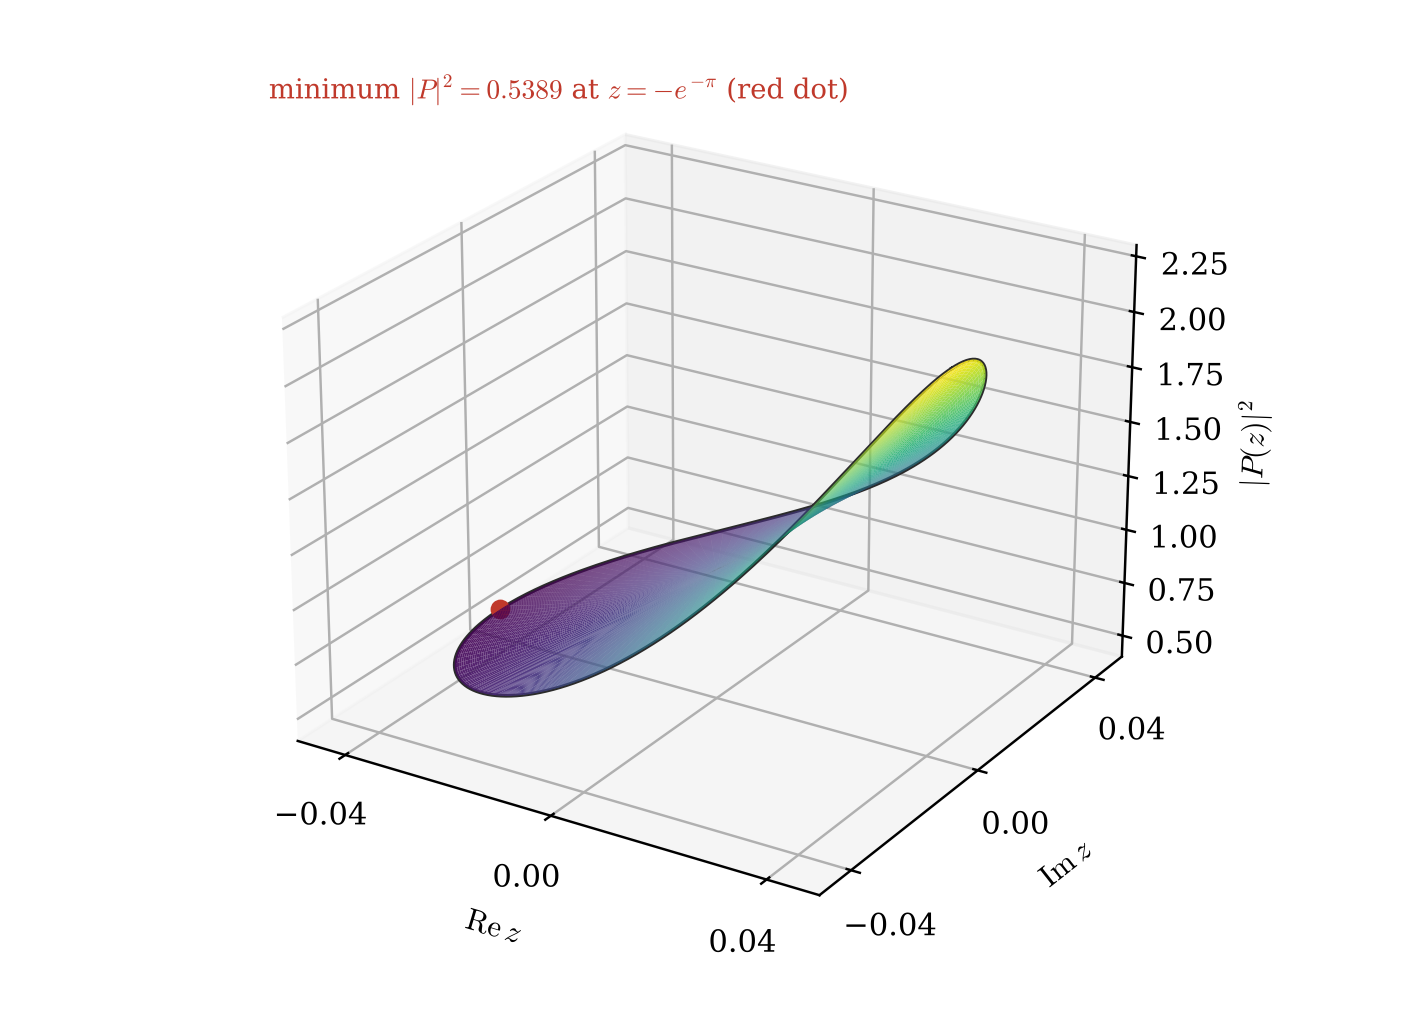
\includegraphics[width=0.78\textwidth]{fig_pdisc.png}
\caption{The surface $|P(z)|^2$ over the disc $|z|\le e^{-\pi}$, where $z=e^{-\pi x+i\theta}$ with $x\ge1$. The rim is the image of $x=1$; the lowest point is $z=-e^{-\pi}$, which corresponds to $x=1$ and $\ell=m$ odd.}\label{fig:pdisc}
\end{figure}

\begin{remark}\label{rem:physics}
The function $1/(\eta(\tau)^8\eta(2\tau)^8)$, whose coefficients are $d_1$, is the generating function of the electric half-BPS degeneracies of the model \cite{Sen08}. Theorem~\ref{thm:model} therefore says that, to leading order, the single-centred index of a quarter-BPS black hole is the extreme Bessel term times the squared modulus of the half-BPS generating function, evaluated at the point $z=e^{-\pi\sqrt D/Q^2+i\pi Q\cdot P/Q^2}$. The positivity of $|P|^2$ is automatic; what has to be proved is that the corrections cannot overturn it, and Proposition~\ref{prop:pmin} gives the room.
\end{remark}
